\documentclass[12pt,a4paper]{article}
\usepackage[utf8]{inputenc}
\usepackage[brazil]{babel}
\usepackage[T1]{fontenc}
\usepackage{amsmath}
\usepackage{graphicx}
\usepackage{booktabs}
\usepackage{geometry}
\usepackage{hyperref}
\usepackage{float}
\usepackage{xcolor}
\usepackage{subcaption}
\usepackage{listings}
\usepackage{helvet}
\renewcommand{\familydefault}{\sfdefault}

\geometry{margin=2.5cm}
\graphicspath{{./figuras/}}

\setcounter{secnumdepth}{0}

\lstset{
    language=R,
    basicstyle=\ttfamily\small,
    keywordstyle=\color{blue},
    stringstyle=\color{orange},
    commentstyle=\color{gray},
    numbers=none,
    frame=single,
    breaklines=true,
    backgroundcolor=\color{gray!10},
    showstringspaces=false
}

\hypersetup{
    colorlinks=true,
    linkcolor=blue,
    filecolor=magenta,
    urlcolor=cyan,
}

\begin{document}

% ============================================================================
% CABEÇALHO
% ============================================================================
\section{}

\textbf{Alunos:} Gabriel Francelino Voidaleski, Lucca Haj Mussi Chella Paranhos Silva

\textbf{Curso:} Tecnologia em Análise e Desenvolvimento de Sistemas (TADS)

\textbf{Disciplina:} Biologia Computacional e Sistemas

\vspace{0.5cm}

Neste trabalho analisamos uma rede biológica usando o conceito de grafos, com o auxílio da biblioteca \texttt{igraph} no R. O objetivo foi transformar os dados de interações em um grafo e, a partir dele, extrair informações sobre a estrutura da rede: quais nós são mais importantes, como a rede está organizada e se existem grupos bem definidos dentro dela.

% ============================================================================
% BASE DE DADOS
% ============================================================================
\section{Base de Dados Escolhida}

\textbf{Fonte:} Network Repository (\url{https://networkrepository.com/})

\textbf{Arquivo utilizado:} \texttt{bio-yeast.mtx}

\textbf{Descrição:} Rede biológica que representa interações entre proteínas de levedura. Cada nó é uma proteína e cada aresta indica que duas proteínas interagem entre si. A rede possui \textbf{1458 nós} e \textbf{1948 arestas}, e pertence à categoria \textit{Biology} do repositório.

% ============================================================================
% ETAPA 1
% ============================================================================
\section{Etapa 1 — Importação e Limpeza}

O arquivo \texttt{.mtx} (formato Matrix Market) começa com linhas de comentário marcadas com \texttt{\%} e depois tem uma linha com as dimensões da matriz. O que nos interessa são as linhas seguintes, cada uma representando uma aresta (par de nós). O código abaixo faz essa leitura, cria o grafo e remove loops e arestas duplicadas:

\begin{lstlisting}
# Ler arquivo .mtx e remover linhas de comentario (%)
linhas <- readLines("bio-yeast.mtx", warn = FALSE)
linhas_sem_comentario <- linhas[!startsWith(linhas, "%")]

# Descartar a primeira linha util (dimensoes da matriz)
dados_brutos <- read.table(text = linhas_sem_comentario[-1], header = FALSE)

# Criar o grafo a partir da lista de arestas
network <- as.matrix(dados_brutos[, 1:2])
grafo <- graph_from_edgelist(network, directed = FALSE)

# Remover loops e arestas multiplas (simplificacao)
grafo <- simplify(grafo, remove.multiple = TRUE, remove.loops = TRUE)

# Verificar se a rede e direcionada
is_directed(grafo)  # FALSE
\end{lstlisting}

A rede é \textbf{não direcionada}, o que faz sentido para interações entre proteínas, onde a relação entre A e B é a mesma que entre B e A.

% ============================================================================
% ETAPA 2
% ============================================================================
\section{Etapa 2 — Caracterização Topológica}

Calculamos os principais indicadores globais da rede para entender sua estrutura geral:

\begin{lstlisting}
vcount(grafo)           # Numero de vertices (ordem)
ecount(grafo)           # Numero de arestas (tamanho)
edge_density(grafo)     # Densidade
diameter(grafo, directed = FALSE, unconnected = TRUE)  # Diametro
transitivity(grafo, type = "globalundirected")         # Transitividade
mean(degree(grafo))     # Grau medio
\end{lstlisting}

\begin{table}[H]
\centering
\caption{Indicadores globais da rede bio-yeast}
\begin{tabular}{ll}
\toprule
\textbf{Indicador} & \textbf{Valor} \\
\midrule
Direcionamento     & Não direcionada \\
Ordem (vértices)   & 1458 \\
Tamanho (arestas)  & 1948 \\
Densidade          & 0,001834 \\
Diâmetro           & 19 \\
Transitividade     & 0,051776 \\
Grau médio         & 2,672154 \\
\bottomrule
\end{tabular}
\end{table}

A densidade de 0,18\% indica uma rede muito esparsa: das conexões possíveis entre os 1458 nós, menos de 1 em cada 500 existe de fato. O diâmetro 19 significa que, no pior caso, são necessários 19 "saltos" para ir de uma proteína a outra. A transitividade (também chamada de coeficiente de agrupamento global) vale 0,052 — um valor bem maior que a densidade, o que indica que vizinhos de um nó tendem a também se conectar entre si mais do que seria esperado em uma rede aleatória. O grau médio de 2,67 mostra que a maioria das proteínas possui poucas conexões diretas, com poucos nós muito conectados. Além disso, remover nós isolados não alterou a ordem da rede, indicando que praticamente todos os vértices participam de alguma interação.

Quanto à classificação como rede de ``mundo pequeno'' (\textit{small world}): redes desse tipo costumam ter diâmetro pequeno e transitividade alta ao mesmo tempo. Aqui, o diâmetro de 19 é relativamente alto para 1458 nós, então a rede não se encaixa bem nessa categoria. A classificação mais adequada é de uma \textbf{rede biológica esparsa e modular}.

% ============================================================================
% ETAPA 3
% ============================================================================
\section{Etapa 3 — Identificação de Atores-chave (Hubs)}

Calculamos duas métricas de centralidade para todos os nós e identificamos os 5 mais importantes em cada uma:

\begin{lstlisting}
# Calcular grau e intermediacao de todos os nos
graus <- degree(grafo)
inter <- betweenness(grafo, directed = FALSE)

# Selecionar os top 5 em cada metrica
top_5_grau <- order(graus, decreasing = TRUE)[1:5]
top_5_inter <- order(inter, decreasing = TRUE)[1:5]
\end{lstlisting}

\textbf{Top 5 por Grau} (número de conexões diretas):

\begin{center}
Nó 147 (56), Nó 819 (38), Nó 98 (30), Nó 567 (29), Nó 844 (29)
\end{center}

\textbf{Top 5 por Intermediação} (Betweenness — quantos caminhos curtos passam pelo nó):

\begin{center}
Nó 819 (225922,23), Nó 844 (148268,95), Nó 98 (122960,35), Nó 147 (104507,89), Nó 595 (83235,45)
\end{center}

\textbf{Discussão do papel estrutural dos hubs:}

Os rankings não são idênticos, o que é bem interessante. Quatro nós aparecem nos dois lists (147, 819, 98 e 844), mas há diferenças:

\begin{itemize}
    \item O \textbf{nó 147} lidera em grau (56 conexões), mas está apenas em 4º lugar na intermediação. Isso indica que ele é um \textbf{conector local} — muito bem conectado dentro do seu grupo, mas não necessariamente uma ponte entre partes distantes da rede.

    \item O \textbf{nó 819} lidera em intermediação, mesmo tendo menos conexões diretas que o nó 147. Isso sugere que ele age como uma \textbf{ponte global} — passa por muitos dos caminhos mais curtos da rede, conectando regiões que de outra forma ficariam mais isoladas.

    \item O \textbf{nó 595} aparece entre os 5 maiores por intermediação, mas não está no top 5 por grau. Esse é o caso mais claro de um nó que, apesar de não ter muitas conexões, ocupa uma posição estratégica na rede — um ``articulador'' entre módulos.
\end{itemize}

Essa diferença entre grau e intermediação revela que, nessa rede, ter muitas conexões nem sempre significa ser o mais importante para a comunicação entre proteínas. A posição estrutural também importa.

% ============================================================================
% ETAPA 4
% ============================================================================
\section{Etapa 4 — Detecção de Comunidades e Visualização}

Para detectar comunidades, usamos o algoritmo de Louvain, que tenta agrupar nós de forma que haja mais conexões dentro dos grupos do que entre eles. A visualização usa o layout Fruchterman-Reingold, onde o tamanho de cada nó é proporcional ao seu grau e a cor indica a comunidade à qual pertence.

\begin{lstlisting}
set.seed(42)
comunidades <- cluster_louvain(grafo)
layout_fr   <- layout_with_fr(grafo, niter = 1500)

# Tamanho dos nos proporcional ao grau
tamanhos_nos <- 2 + 7 * (graus - min(graus)) / (max(graus) - min(graus))

# Cor dos nos por comunidade
membros  <- membership(comunidades)
paleta   <- hcl.colors(length(unique(membros)), palette = "Dark 3")
cores_nos <- paleta[membros]

plot(grafo, layout = layout_fr,
     vertex.size  = tamanhos_nos,
     vertex.color = cores_nos,
     vertex.label = NA)
\end{lstlisting}

% ============================================================================
% VISUALIZAÇÕES
% ============================================================================
\section{Visualizações Produzidas}

\subsection{Rede completa com comunidades (Etapa 4)}

\begin{figure}[H]
\centering
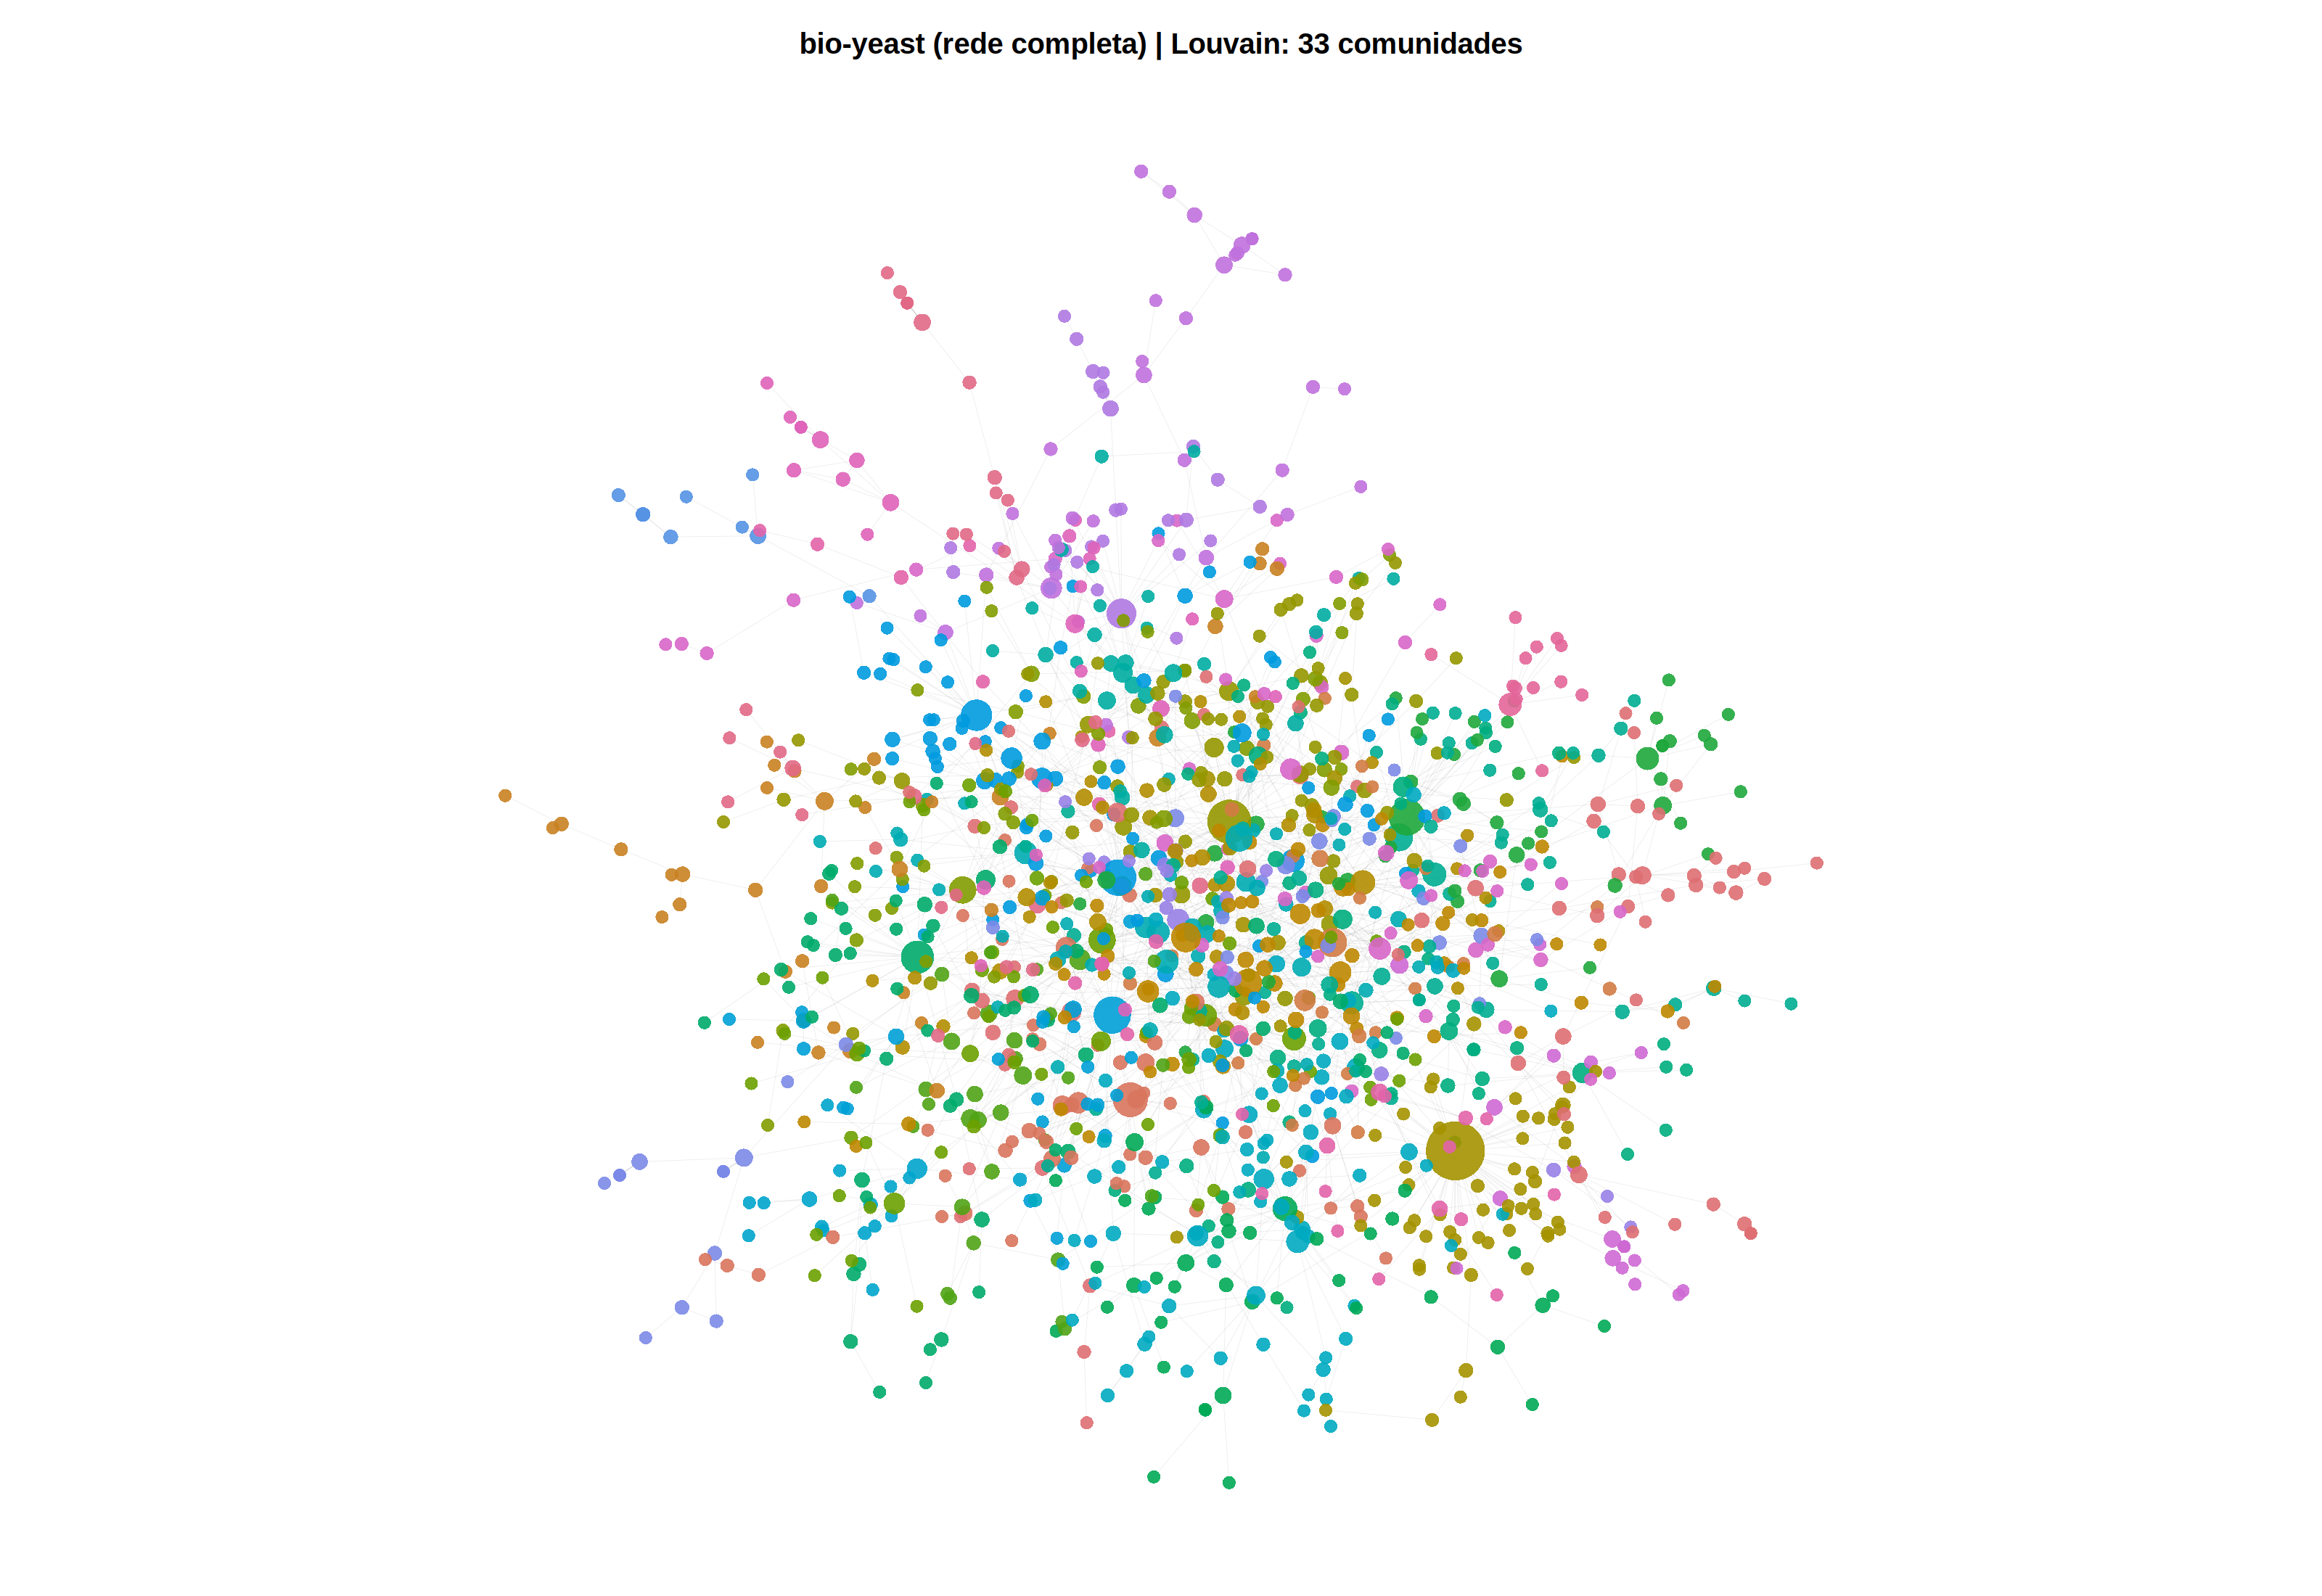
\includegraphics[width=0.98\textwidth]{rede_completa_comunidades_200ppi.png}
\caption{Rede completa bio-yeast com comunidades detectadas pelo algoritmo de Louvain. O tamanho de cada nó é proporcional ao seu grau e a cor indica a comunidade. Layout: Fruchterman-Reingold.}
\end{figure}

\subsection{Componente gigante com hubs destacados}

\begin{figure}[H]
\centering
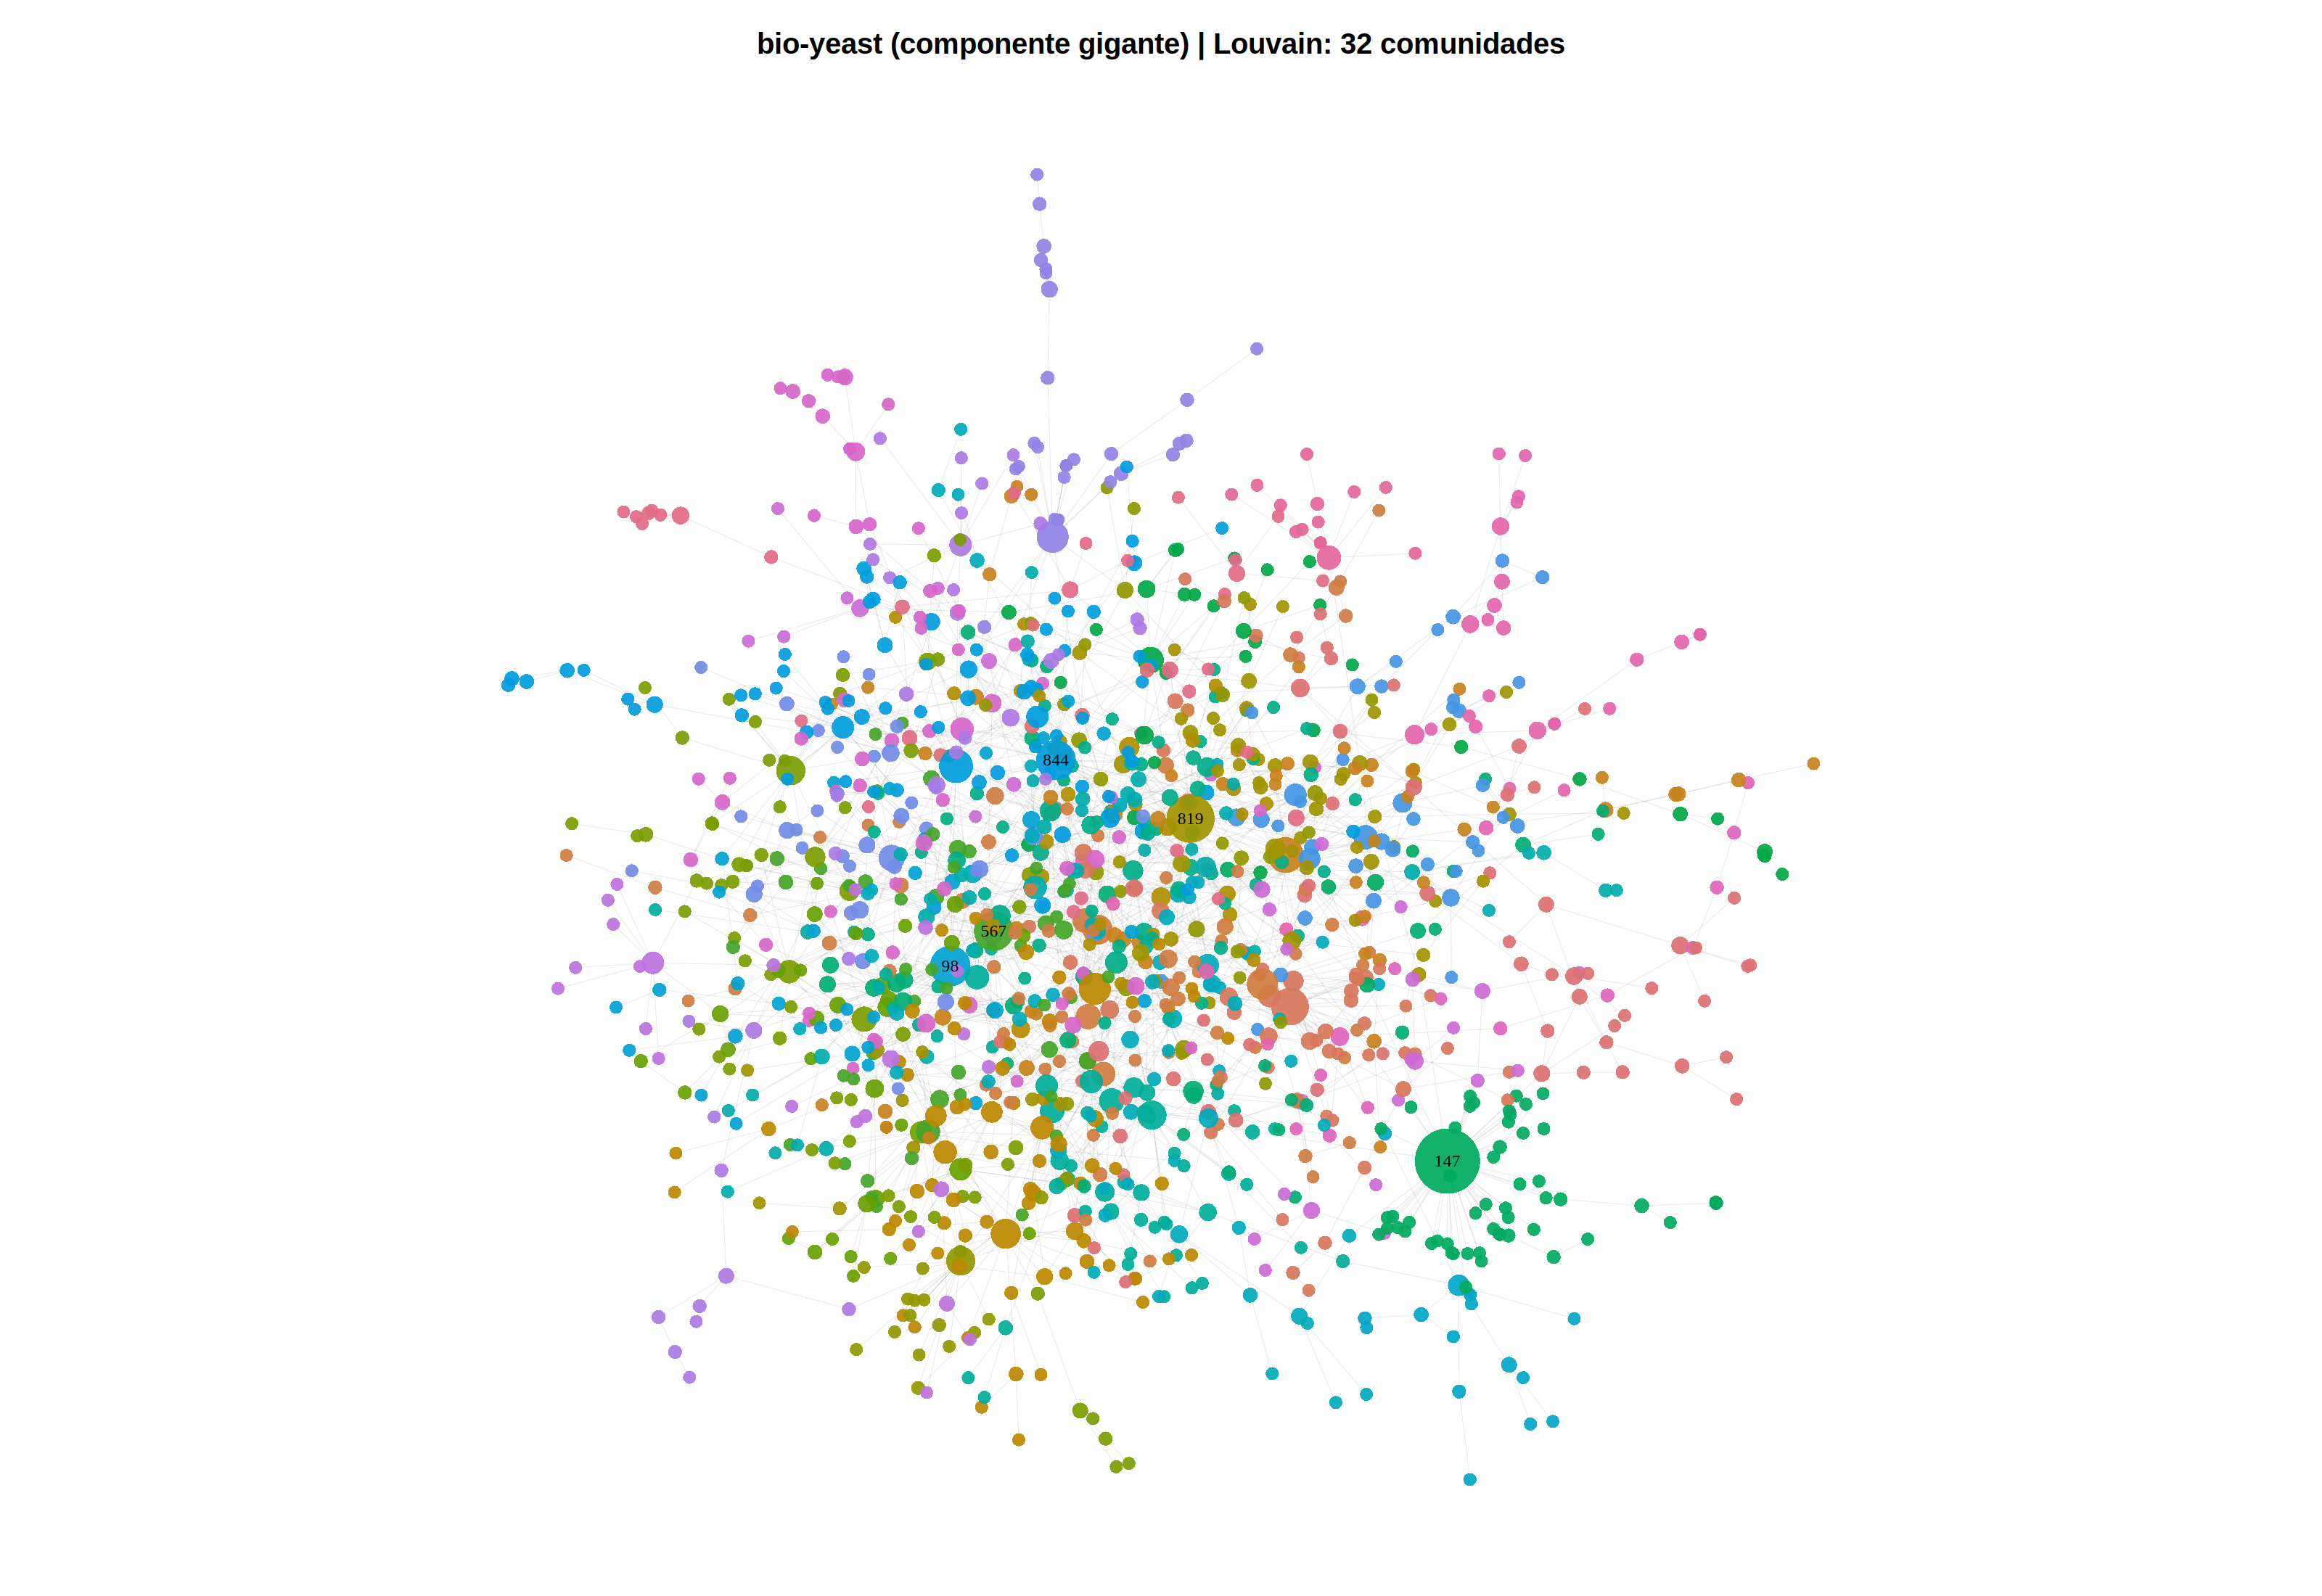
\includegraphics[width=0.98\textwidth]{componente_gigante_comunidades_200ppi.png}
\caption{Componente gigante da rede, com os 5 hubs de maior grau identificados por rótulo. Facilita a visualização da posição central desses nós.}
\end{figure}

\subsection{Comparativo dos hubs por grau, intermediação e distribuição}

\begin{figure}[H]
\centering
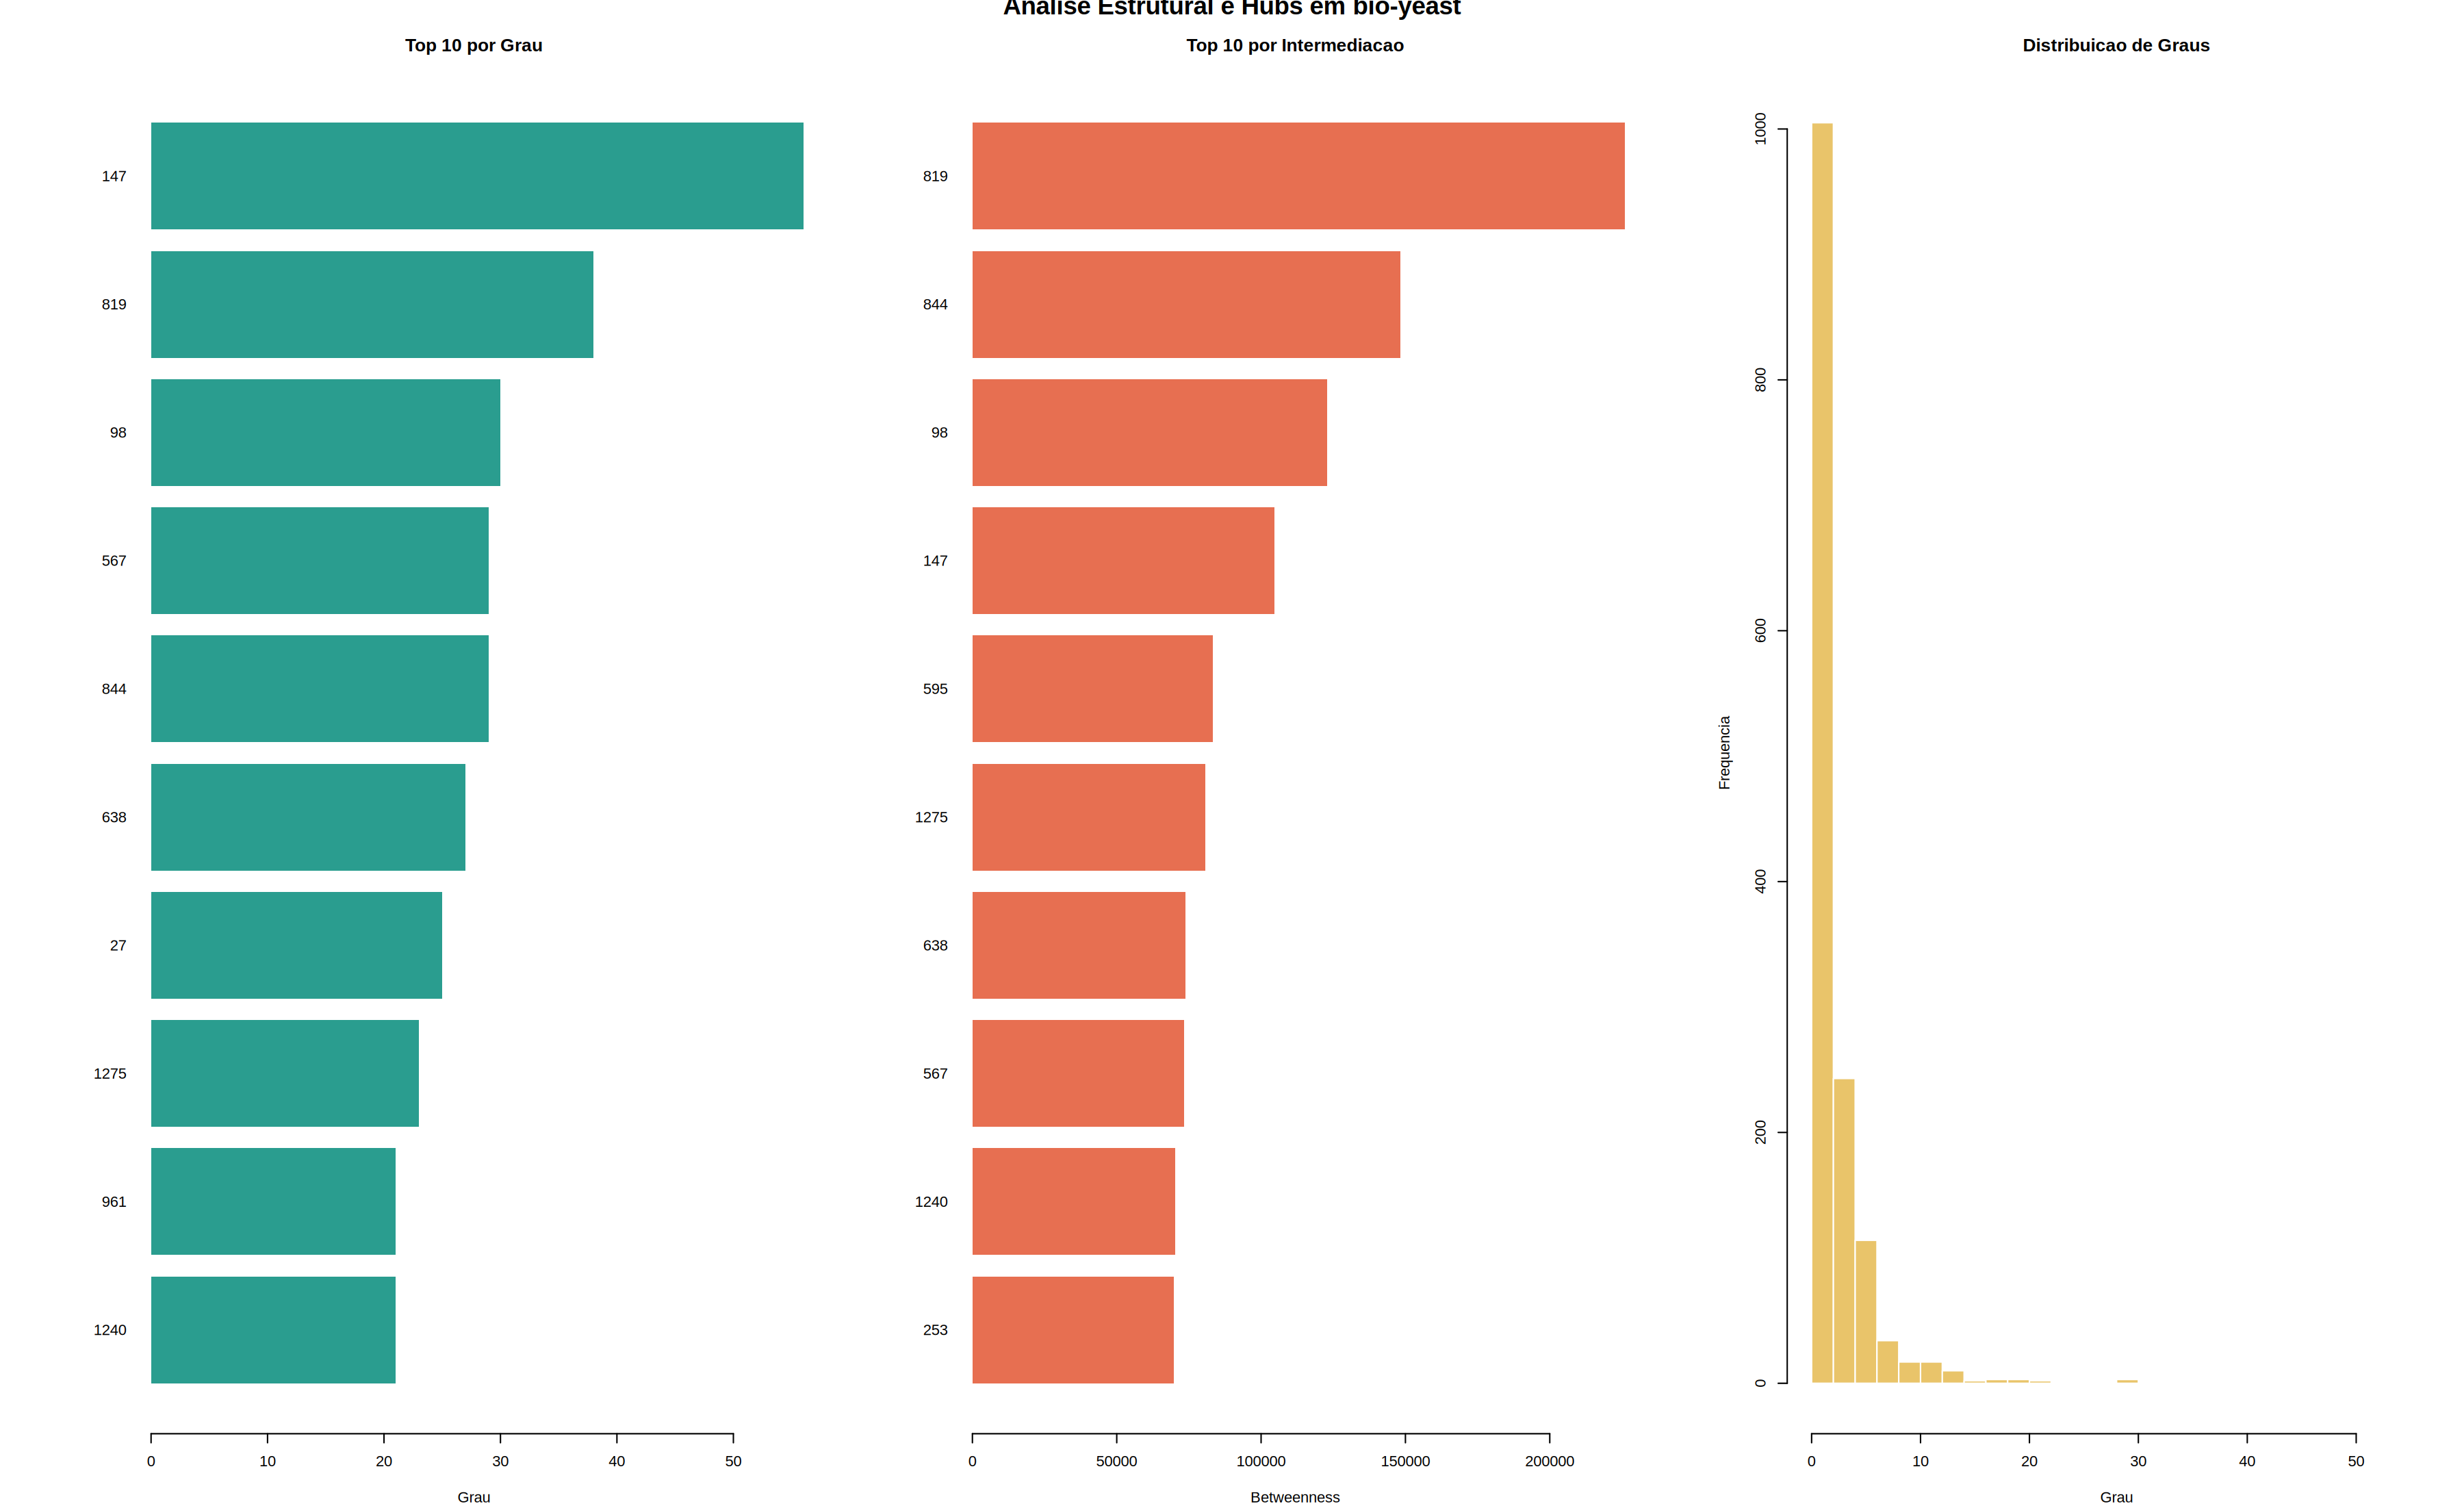
\includegraphics[width=0.98\textwidth]{top_hubs_grau_intermediacao_200ppi.png}
\caption{Top 10 nós por Grau (esquerda), por Intermediação/Betweenness (centro) e distribuição de graus (direita). A comparação visual deixa clara a diferença entre os dois rankings e a concentração de nós com baixo grau.}
\end{figure}

% ============================================================================
% ANÁLISE FINAL
% ============================================================================
\section{Análise Final}

\textbf{Tipo de rede e classificação estrutural}

A rede bio-yeast é uma rede biológica de interações proteína-proteína (PPI) esparsa e modular. A densidade muito baixa (0,18\%) mostra que cada proteína interage com apenas uma pequena fração das demais, o que é típico de redes biológicas. O coeficiente de transitividade (0,052), bem mais alto que a densidade, indica que proteínas que interagem com uma mesma terceira proteína também tendem a interagir entre si com mais frequência do que seria esperado ao acaso. O diâmetro de 19 mostra que a rede não é compacta o suficiente para ser classificada como \textit{small world}: apesar dos agrupamentos locais, os caminhos entre partes distantes da rede são relativamente longos. O grau médio de 2,67 e o histograma de graus reforçam a presença de poucos hubs muito conectados frente a muitos nós de baixo grau.

\textbf{Análise dos hubs}

Como discutido na Etapa 3, os nós com maior grau não são exatamente os mesmos com maior intermediação. Isso revela duas funções estruturais distintas: alguns nós são importantes porque têm muitas conexões diretas (conectores locais, como o nó 147), enquanto outros são importantes porque estão em posições estratégicas entre diferentes partes da rede (pontes globais, como o nó 819). A presença do nó 595 — alto em intermediação, mas fora do top 5 em grau — é um exemplo claro de que a posição na rede pode ser mais determinante do que a quantidade de conexões.

\textbf{Interpretação das comunidades}

Olhando para as imagens geradas, as comunidades fazem sentido visual: é possível ver claramente grupos de nós mais próximos uns dos outros e com cores distintas, separados por poucas conexões entre os grupos. No contexto biológico, essas comunidades provavelmente representam \textbf{conjuntos de proteínas que participam de processos celulares semelhantes} — por exemplo, proteínas envolvidas na divisão celular, no reparo de DNA ou no metabolismo energético podem aparecer mais conectadas entre si do que com proteínas de outras funções. Isso está alinhado com o que a literatura aponta para redes PPI de levedura: a modularidade funcional é uma característica esperada.

% ============================================================================
% CONCLUSÃO
% ============================================================================
\section{Conclusão}

A análise da rede bio-yeast passou pelas quatro etapas do enunciado: importação e limpeza dos dados, cálculo das métricas globais, identificação dos nós mais importantes e detecção de comunidades com visualização. Os resultados mostraram uma rede esparsa, com agrupamentos locais bem definidos e hubs com papéis estruturais distintos. A diferença entre os rankings de grau e intermediação foi o ponto mais interessante da análise, mostrando que a importância de um nó em uma rede não depende apenas de quantas conexões ele tem, mas também de onde ele está posicionado na estrutura geral.

\end{document}
